\section{Cut and count analysis}

\subsection{optimization} 

The same varibale set as used for MVA training is employed.
The Simulating Annealing method in TMVA is used.
The cuts are selected such that the selection signal efficiency matches that of the BDT.

\begin{verbatim}
Barrel:
	 5.66532 < "pt" <= 108.395
	 -1.34013 < "eta" <= 1.90538
	 13.4938 < "fls3d" <= 113.735
	 -0.00248177 < "alpha" <= 0.0554104
	 -0.000113258 < "maxdoca" <= 0.0140014
	 -0.00089438 < "pvip" <= 0.055899
	 0.0869982 < "pvips" <= 4.19143
	 0.425172 < "iso" <= 1.03777
	 0.00903932 < "docatrk" <= 0.196985
	 -0.0104609 < "closetrk" <= 8.94004
	 -0.0949024 < "chi2dof" <= 5.55102

Endcaps:
	6.81716 < "pt" <= 58.3142
	-2.26185 < "eta" <= 2.35863
	12.9774 < "fls3d" <= 122.734
	-0.00186433 < "alpha" <= 0.236627
	-0.000172019 < "maxdoca" <= 0.0192271
	0.000376399 < "pvip" <= 0.0379179
	0.0897054 < "pvips" <= 1.20388
	0.59898 < "iso" <= 1.2262
	0.011315 < "docatrk" <= 0.163787
	-0.196135 < "closetrk" <= 17.3713
	-0.0797694 < "chi2dof" <= 3.64842
\end{verbatim}

\subsection{blinded results}


\begin{figure}[!h]
  \centering
  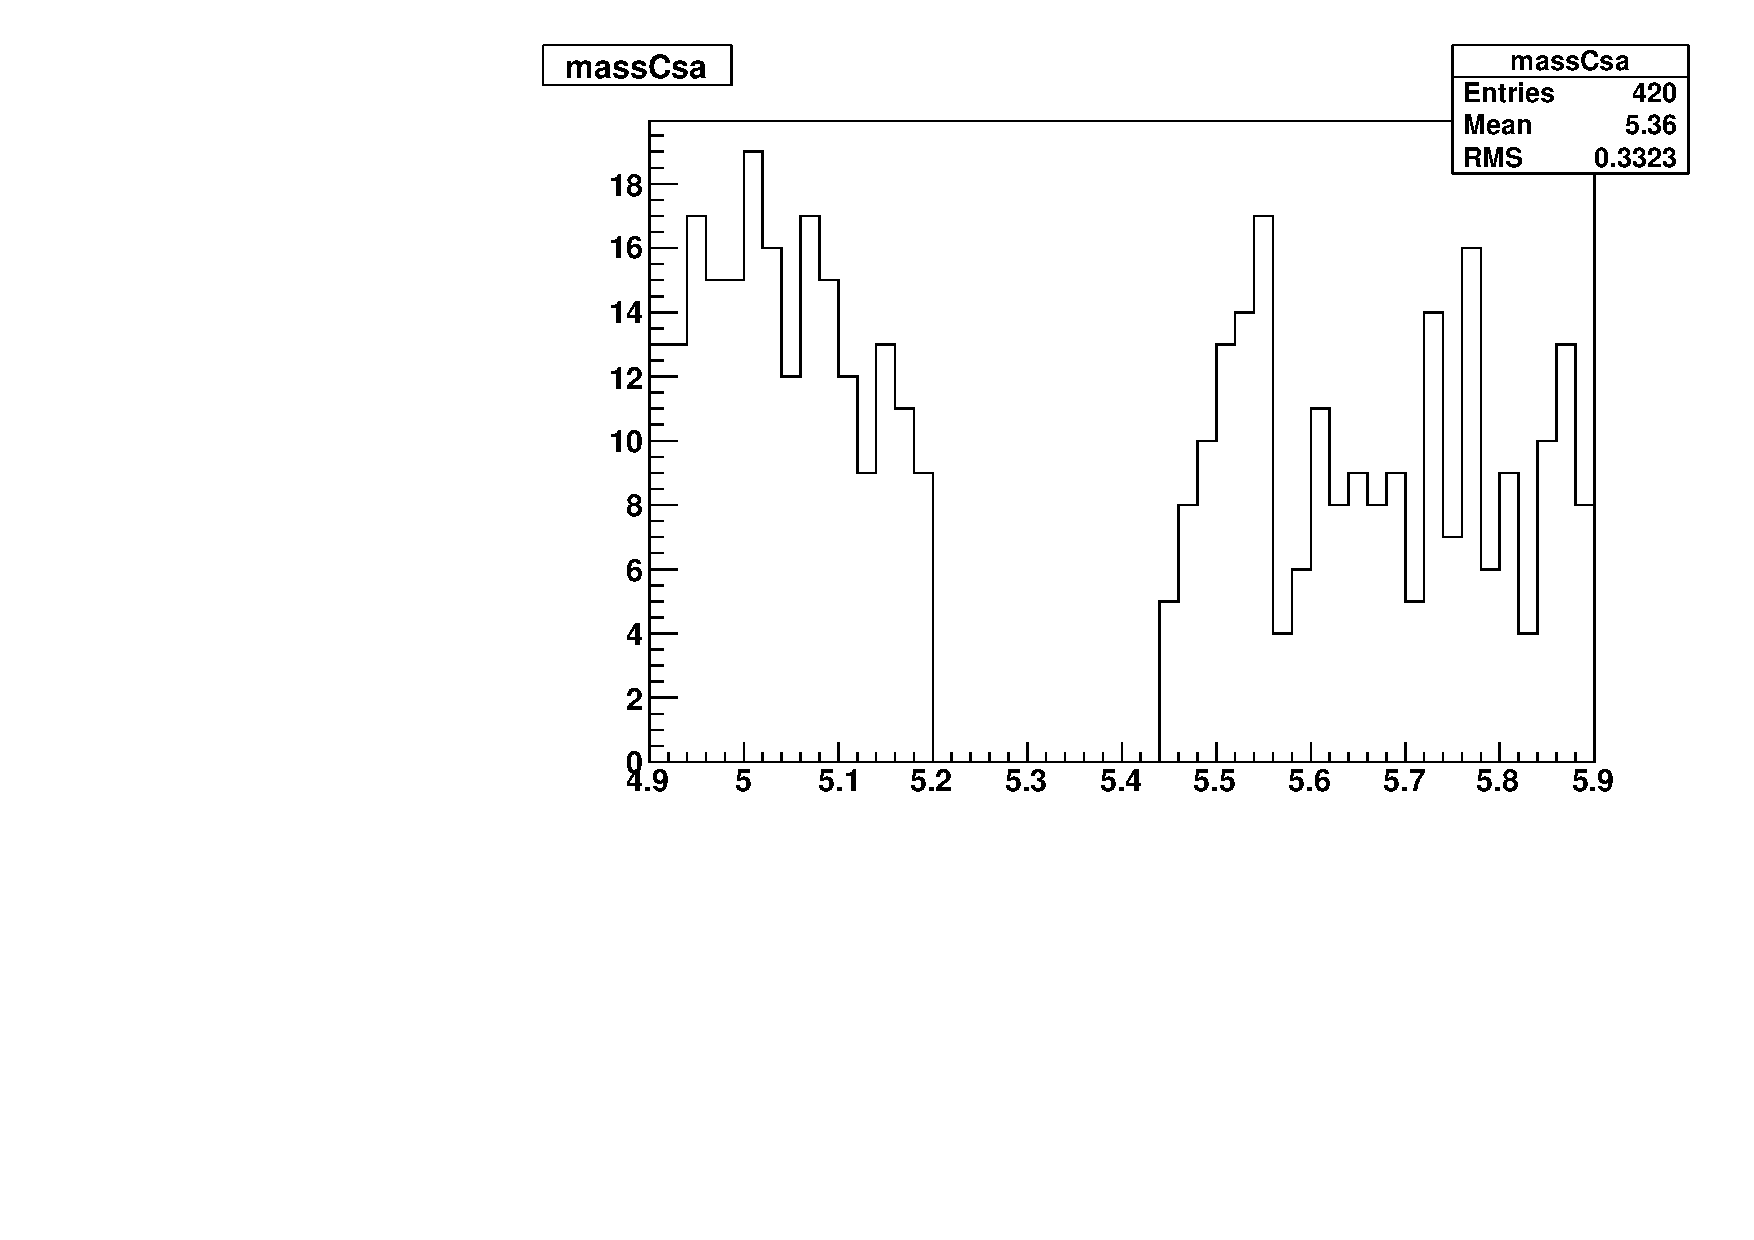
\includegraphics[width=0.45\textwidth]{Figures/cnt/SA_barrel_mass}
  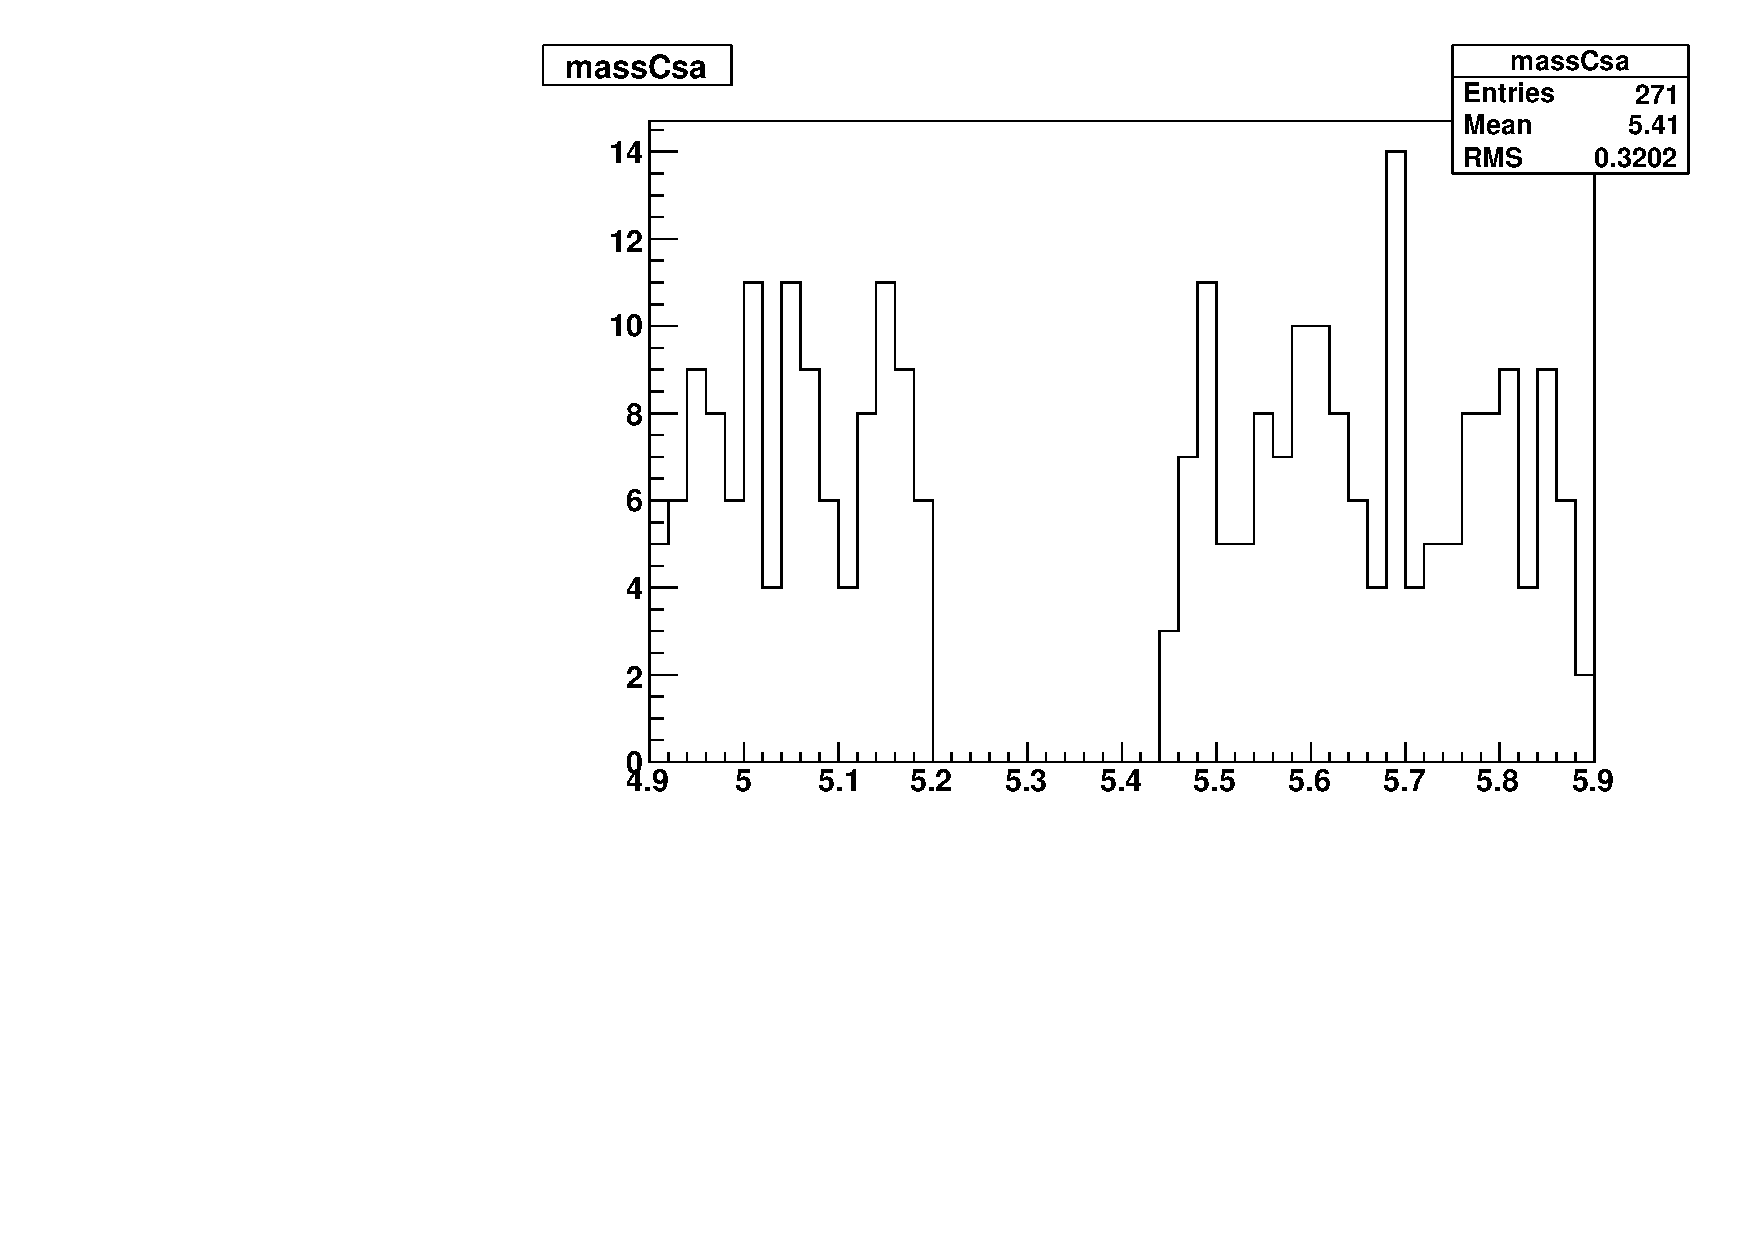
\includegraphics[width=0.45\textwidth]{Figures/cnt/SA_endcaps_mass}
\caption{Blinded cut results for barrel (left) and endcaps (right).}
\end{figure}


\subsection{unblind}

\begin{figure}[!h]
  \centering
  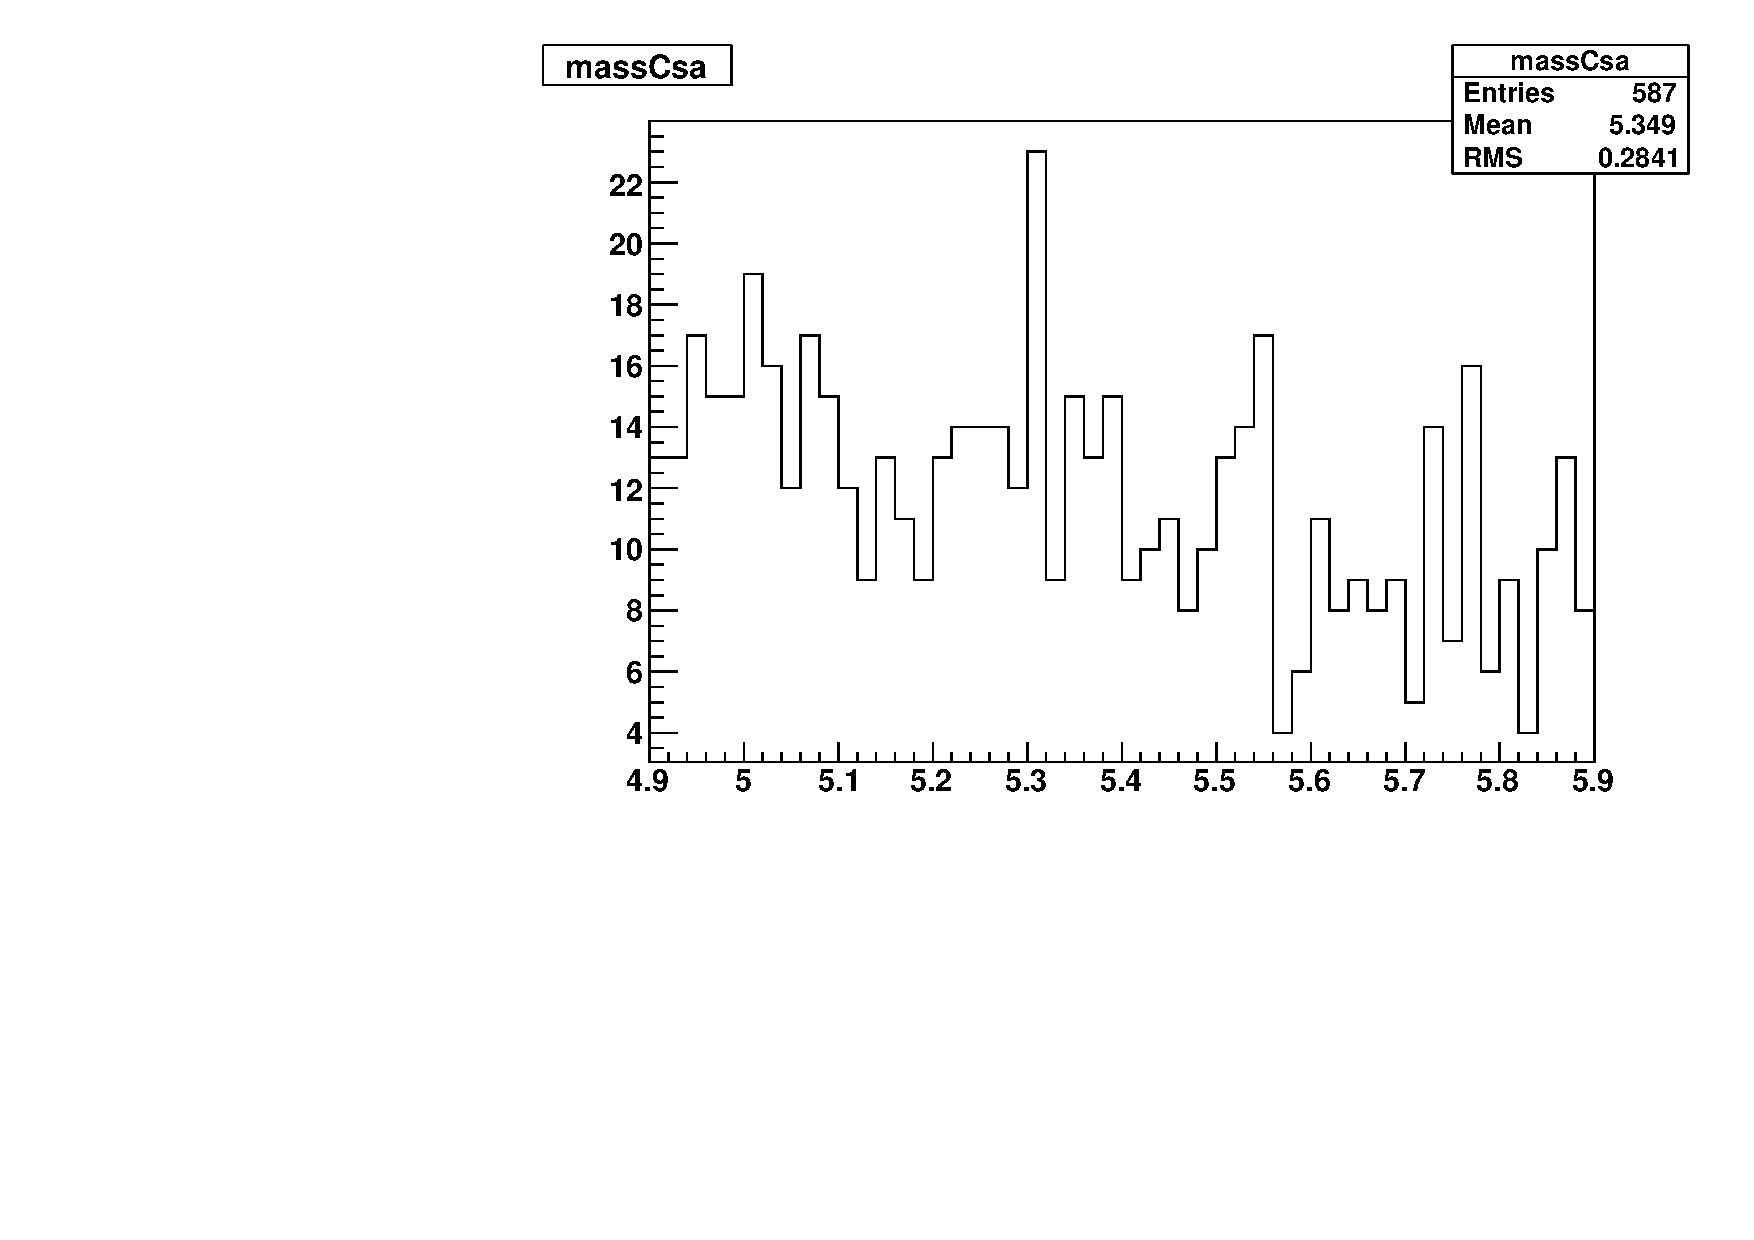
\includegraphics[width=0.45\textwidth]{Figures/cnt/SA_barrel_mass_unblind}
  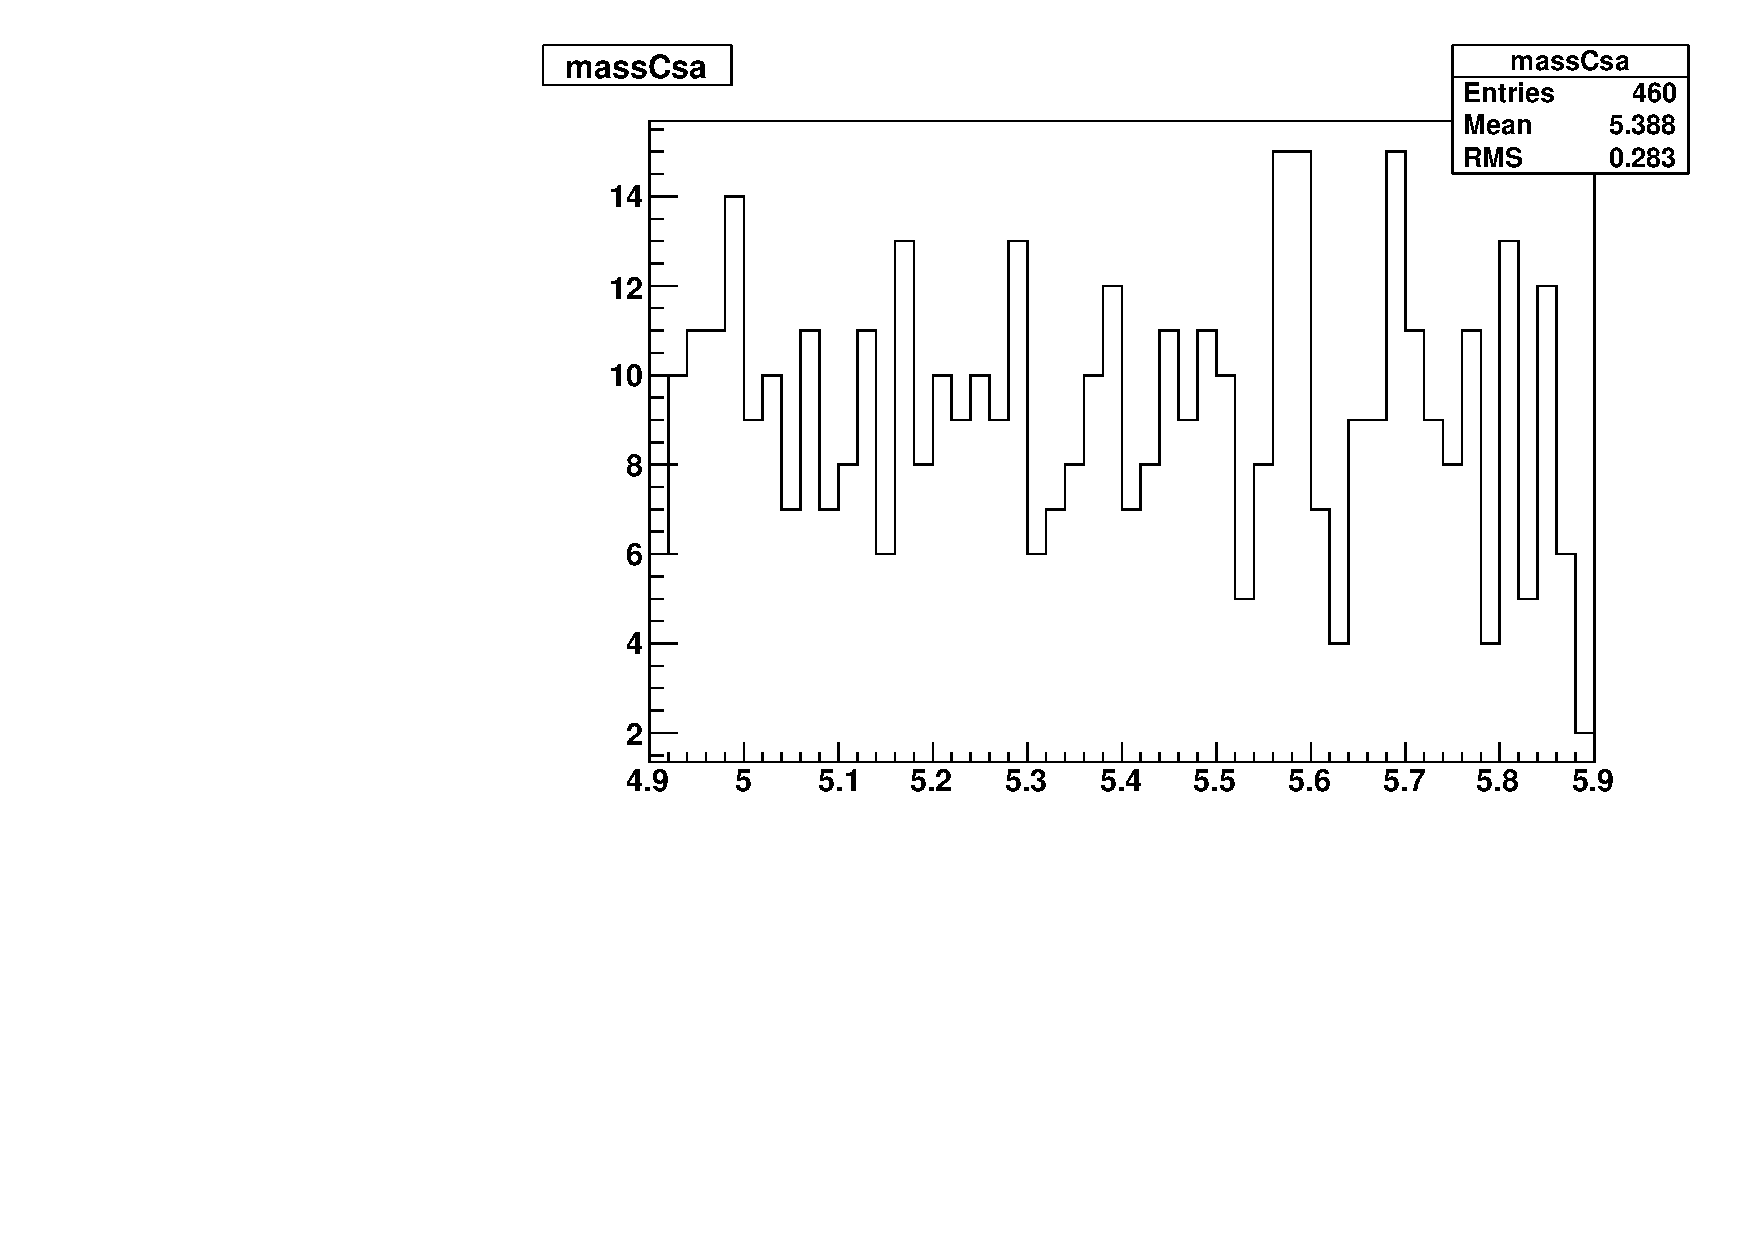
\includegraphics[width=0.45\textwidth]{Figures/cnt/SA_endcaps_mass_unblind}
\caption{Unblinded cut results for barrel (left) and endcaps (right).}
\end{figure}
